\documentclass[a4paper,english]{article}
%Scandinavian alphabet
\usepackage{babel}
\usepackage[latin1]{inputenc}
\usepackage{epsfig,textcomp,supertabular}

%Citation style 
\usepackage[round,authoryear]{natbib}
\hyphenation{Linden-mayer meta-bolism} 

\title{Enhancing the Modeling Capabilities of LIGNUM with Lindenmayer systems}

\author{Jari Perttunen
        \footnote{Corresponding author, email: jari.perttunen@metla.fi.}
        \footnote{Finnish Forest  Research Institute, Vantaa Research
                  Station, P.O.Box 18, 01301 Vantaa, Finland.}
\and Radek Karwowski\footnote{University of Calgary}
\addtocounter{footnote}{-1}
\and Przemyslaw Prusinkiewicz\footnotemark
\addtocounter{footnote}{-3}
\and Risto Siev�nen\footnotemark
}


%suggested running title
\markright{Perttunen et al. -- Lindenmayer systems in LIGNUM}
\pagestyle{myheadings}
%Double line space if needed
%\linespread{1.65} 

%This is how to get around nonnumerical years (xxxxa,xxxxb, etc.)
%with natbib when the author has been really energetical. 
\defcitealias{kurth:em94}{Kurth,~1994b}

%Equation numbers in brackets
%\makeatletter
%\renewcommand\@eqnnum{\hb@xt@.01\p@{}%
%                      \rlap{\normalfont\normalcolor
%                        \hskip -\displaywidth[\theequation]}}
%\makeatother

\begin{document}

\maketitle
\pagebreak

\abstract{
  
  LIGNUM  is  a   functional-structural  tree  model  that  represents
  coniferous and broad-leaved trees  with four modelling units closely
  resembling  the  real  structure  of  trees.   The  units  are  tree
  segments,  the  tree axes,  branching  points  and buds.   Metabolic
  processes are  explicitly related to  the structural units  in which
  they are  taking place.  Here we  enhance the model  LIGNUM with the
  possibility to formally describe  the architectural development of a
  tree with Lindenmayer systems.
  
  We give sample applications of  the system to model single trees and
  forest stand.  Finally we discuss our approach  and its consequences
  for the future development of the model.

\bf Key words\rm: LIGNUM, Lindenmayer systems, functional-structural tree model.  
}

\section{Introduction}
An increasing number of models  (see e.g. Annals of Forest Science vol
57 no.  5/6) try to determine  dynamics and growth  of woody perennial
plants by assessing physiological processes in their three dimensional
arborescent  form.    Physiological  processes  involve   for  example
photosynthesis of  the foliage, respiration, flow  of water, nutrients
or hormones and allocation  of nutritive substances.  The structure of
the tree and  its changes in time is described  for example with state
variables representing different  aggregated tree compartments or with
detailed modelling  components faithful to  botanical or morphological
units of  plants. Such  models have been  called functional-structural
(FSTM).

W.  Kurth has  proposed a  model triangle  \citep{kurth:94b} arranging
existing modelling approaches in  forestry into three categories based
on the  emphasis in the modeling approaches  (structure vs.  function,
single tree vs. forest  stand).  Accordingly there are practically two
ways to construct an FSTM  \citep{sievanen:00}.  One can start from an
architectural  model   \citep{jaeger:92,kurth:94}  adding  functional,
physiological details into it.  The second approach is to begin with a
process  based  physiological  model  \citep{makela:86,  landsberg:86,
sievanen:93} and extend it with structural details.

Linking these  two kinds of  models together rises the  question about
the suitable way of  expressing them. Physiological models usually are
realized  with  the  aid   of  differential  or  difference  equations
\citep{landsberg:86}  whereas architectural  models  apply Lindenmayer
systems  \citep{kurth:99,pp:90}  or  other  formalisms. Would  a  FSTM
combine those means or rely on either of them?

The model LIGNUM  approaches FSTM from the physiological  side; it is a
single  tree  model  \citep{perttunen:96}  faithful  to  process-based
modelling  \citep[see  e.g.][]{nikinmaa:92, sievanen:93,  makela:97-1}
but  instead  of  aggregated  tree  parts  it  has  three  dimensional
description of the  above ground part of the  tree.  LIGNUM includes a
detailed    model    of    self-shading    within   a    tree    crown
\citep{perttunen:96, perttunen:01} from which the radiation regime for
photosynthesis in different parts of the tree can be computed.  If the
photosynthates produced exceed respiration costs the net production is
allocated to the growth of new  parts. LIGNUM has been applied to both
coniferous   \citep{perttunen:96,lo:99}   and   broad   leaved   trees
\citep{perttunen:01}. The main focus in LIGNUM has been on the
functional  part  of  the  model;  less  emphasis  has  been  paid  to
structural  development, and  the model  does not  include  any formal
method to define the architectural development of the tree structure.

Since the pioneering work  by \citet{honda:71} there exist methods for
treating   plant  architecture   in  models   in  an   efficient  way.
Lindenmayer-systems or L-systems for  short \citep{pp:89} are the most
widely  used  method  to   treat  plant  architecture  although  other
formalisms   also  exist \citep[e.g.][]{dereffye:97,   godin:99}.
L-systems   were  invented   in   by  Aristid   \citet{lindenmayer:68,
  lindenmayer:71} and were initially meant to describe the development
of  multicellular organisms.  L-systems  are string  rewriting systems
and their research  is concerned with the question  what phenomena can
be   described  with   formal  languages.    The  theory,   tools  and
applications using  L-systems framework for modeling  plants and their
environment have been  developed by Prusinkiewicz \citep{pp:89,pp:92},
Kurth  \citep{kurth:94} and other  scientists.  The  ubiquitous theory
and the progress in L-systems  in modelling plants and trees until the
end   of  '90's   is  well   documented  in   \citet{pp:90,pp:99}  and
\citet{kurth:99}.

We describe in the following  how the model LIGNUM has been interfaced
with   L-systems   for   specifying   formally  and   rigorously   the
architectural   development  of  trees   and  thereby   improving  the
applicability and  ease of using this  FSTM.  The goal  is achieved by
using the language L that  is an extension of L-systems \citep{pp:99a}.
Based on the definition of  L, R.  Karwowski has created the original
parser of L and  has implemented the language L+C \citep{karwowski:02}
including  further  improvements  not   present  in  L,  most  notably
productions with multiple successors and the concept of new context
\citep{karwowski:03} to allow fast linear time information transfer in
the simulated plant.

We first  present the use of L  in LIGNUM based on  the similarity how
LIGNUM and bracketed L-systems represent branching structures of trees
\citep{perttunen:96, perttunen:01}.  Second, we implement an algorithm
that  translates  the bracketed  string  of  symbols  in L  to  LIGNUM
representation of  trees (Section \ref{sec:pine}).   Third, we provide
communication  mechanism  between  the  L-string and  LIGNUM  (Section
\ref{sec:LtoLignum}) and give two  sample applications, Scots pine and
bearberry.   We present simple  language construct  that allows  us to
model   group  of  plants   each  with   its  own   L-system  (Section
\ref{sec:namespace}).   Finally,  we  discuss  our  approach  for  its
consequences to the future development of LIGNUM in modeling trees and
forest stands.


\section{Structural units of LIGNUM}
LIGNUM is intended as a generic modelling tool for both coniferous and
hardwood trees.  Different tree  species can be simulated by assessing
descriptions of  metabolism, structural dynamics of  birth, growth and
senescence,  and by  implementing  branching rules  for distinct  tree
architectures  \citep{perttunen:96,  perttunen:01}.   Here we  present
shortly the main model features to understand how LIGNUM is adapted to
use L-systems.

The metabolic  activities incorporated in LIGNUM  are interception and
attenuation  of  photosynthetically  active  solar radiation  in  tree
crown,  photosynthetic  production,  respiration and  partitioning  of
growth  between  new parts  and  existing  structure. Some  mechanical
interactions,  like bending of  branches or  collision of  branch tips
have also been implemented.

LIGNUM represents the three-dimensional  above ground part of the tree
with  four  structural  units  called  tree  segment  (TS),  bud  (B),
branching point (BP) and axis (A). The most important functioning unit
is the cylindrical tree segment, section of woody material between two
branching points.  For  conifers needles are at the  moment modeled as
cylindrical  layers   of  foliage  surrounding   tree  segments.   For
deciduous species leaves attached  to tree segments are considered and
studied explicitly  using simple geometric  form like ellipse  as leaf
shape.  Branching  point and axis  capture the recursive  structure of
the tree  crown.  Branching point is  a set of  axes and an axis  is a
sequence of tree segments, branching points and terminating bud.

An axis  is implemented as  a list. For  example the main axis  of the
model tree for coniferous species (\ref{fig:model} ) consists of three
tree segments, three branching points and the terminating bud:

\begin{equation}
[TS_0,BP_1,TS_2,BP_3,TS_4,BP_5,B_6]
\end{equation}

A branching  point is implemented as  list of axes. In  the model tree
the branching points contain two axes  each. Thus the main axis can be
written:

\begin{equation}
[TS_0,[[A,A]],TS_2,[A,A],TS_4,[A,A],B_6]
\end{equation}

Finally, the structure of the whole model tree is expressed as:

\begin{equation}\label{eq:tree}
[TS_0,[[TS,[],B],[TS,[],B]],TS_2,[[TS,[],B],[TS,[],B]],TS_4,[[B],[B]],B_6]
\end{equation}

The two empty  lists ([]) for branching points  denote no axes forking
off maintaining the structural integrity of the model.


\section{Basics of L-systems}

Mathematically L-systems  are parallel rewriting  systems operating on
strings of symbols. An L-system  is defined by an alphabet of symbols,
a  set of  rewriting rules  called productions  and an  initial string
called axiom. In a production  written as $a \rightarrow S$ the symbol
$a$  is   called  predecessor  and  the  string   $S$  successor.   In
context-free  L-systems  predecessor's   context  does  not  influence
production  application.  In  context-sensitive  L-systems written  as
$S_l < a  > S_r \rightarrow S$, the symbol $a$  can produce string $S$
if and  only if  $a$ is  preceded by string  $S_l$ (left  context) and
followed  by string  $S_r$ (right  context).  For  example  define the
alphabet of three  symbols $O$, $X$ and $S$ and  set of following nine
rules:
\begin{equation}\label{eq:ca110}
\begin{array}{lll}
1:O < O > O \rightarrow O & 2:O < O > X \rightarrow X &
3:O < X > O \rightarrow X \\ 
4:O < X > X \rightarrow X & 5:X < O > O \rightarrow O&
6:X < O > X \rightarrow X \\
7:X < X > O \rightarrow X & 8:X < X > X \rightarrow O & 
9:S > O \rightarrow SO
\end{array}
\end{equation}
enlisting the $2^3$  possible ways of $O$ and $X$  to interact and the
ninth rule expanding the string.  Starting from the axiom $SOOOXO$ the
first four  strings produced by the L-system  are $SOOOXO$, $SOOOXXO$,
\linebreak $SOOOXXXO$ and $SOOOXXOXO$.

In plant modeling  context the symbols of the  alphabet in an L-system
represent the units (internodes, leaves, flowers etc.)  of the growing
organism relevant to modeling approach and the string of symbols their
topological ordering.  To be able to generate the branching structures
dominant in plant world the notion of strings with brackets (literally
denoting  begin and  end  of branch  with  '[' and  ']') or  bracketed
L-systems   was   already    present   in   the   original   formalism
\citep{lindenmayer:68}. To describe the geometry and for the graphical
interpretation  of  the   model  structures  \citet{pp:86}  introduced
L-system  symbols  as  instructions  controlling a  LOGO-style  turtle
\citep{abelson:82} in three dimensions,  hence the adopted name Turtle
graphics.


\section{Integrating the L language and LIGNUM}\label{sec:pine}

To model tree structures with L as in LIGNUM let the module $F$ denote
a tree segment and designate module  $B$ for a bud.  Given the modules
for turtle graphics and branching we can now describe the topology and
geometry of  the tree structures  of LIGNUM (Eq.   \ref{eq:tree}) with
rules of the  L language.  To accommodate L with  LIGNUM we first need
to construct an algorithm that translates strings of L into structural
units  of  LIGNUM   (Section  \ref{sec:LToLignum}).   Second,  as  the
metabolism  implemented  in  LIGNUM   will  act  on  structural  units
(segments  and  buds  most  notably)  and  produce  changes  in  their
physiological states,  in their dimensions  and in their  positions in
space  accordingly, this  information  must be  transferred to  turtle
symbols  and module  $B$ as  this is  necessary in  rewriting (Section
\ref{sec:LignumToL}).

We present an  algorithm that translates strings of  L into structural
units of LIGNUM  with the aid of an example with  Scots pine.  We have
programmed  in  L  the  architectural  development of  Scots  pine  in
approximately  the same  way as  it is  in the  LIGNUM  simulations of
\citet{perttunen:96, perttunen:98}; the L program is shown in Appendix
\ref{sec:L1}.  In the program the module $B(A,L)$ represents a bud. In
each iteration  the apical bud ($A  = 1$) moves forward  by the length
$L$ and produces  four new side branches.  The branches  ($A > 1$) are
similar, but only two more side branches are created.  Branching stops
after the third order ($A > 3$), but the extension continues. Also, as
$A$ records  branching it is updated  as new branches  are added. When
the development starts  from the main axis consisting  of one segment,
branching point and bud, the string after two iterations is

\begin{eqnarray}\label{eq:pine2}
\lefteqn{F\;[] \;F \; [F[B][B]B]\;[F[B][B]B]\;[F[B][B]B]\;[F[B][B]B] \nonumber }\\
\lefteqn{F \; [B][B][B][B]\; B}
\end{eqnarray}
where symbol  [ denotes $SB()$ and  ] denotes $EB()$,  the modules for
turtle rotations are  not shown, and the arguments  of the modules $B$
and $F$ are dropped.

\subsection{From L to LIGNUM}\label{sec:LToLignum}

We can now  outline a straightforward algorithm to  convert the string
of symbols in L to structural units in LIGNUM using Eq. \ref{eq:pine2}
as a  specific example.  The  algorithm is based on  first recognizing
the main axis  of the tree, then finding the  other axes (branches and
sub-branches), and finally grouping them together as branching points.

First, the  symbol $F(s)$ in  Eq.  \ref{eq:pine2} is interpreted  as a
tree  segment of length  $s$.  The  symbol $B$  corresponds to  a bud.
Each consecutive set of $n$ branches between two $F$ symbols will be a
branching  point with  $n$ axes.   The string  in  Eq.  \ref{eq:pine2}
first  becomes the  main  axis with  three  segments, three  branching
points and the terminating bud:

\begin{equation}
[TS, BP, TS, BP, TS, BP, B]
\end{equation}

The  last two  branching  points  contain four  axes  each, the  first
branching point being empty:

\begin{equation}
[TS, [], TS, [A,A,A,A], TS, [A,A,A,A], B]
\end{equation}

Finally, recursively constructing the axes we get:
\begin{eqnarray}
\lefteqn{[TS, [], TS,[TS,[[B],[B]],B],\ldots, [TS,[[B],[B]],B]], \nonumber} \\
\lefteqn{\;TS, [[B],[B],[B],[B]], B]}
\end{eqnarray}

The current status  of the turtle that is  updated according to turtle
commands in  the string  defines the position  and orientation  of the
tree compartments in LIGNUM.

The structural development of the tree described in L does not require
the regeneration of a LIGNUM representation of trees (deleting the old
tree and  creating a  new one) after  each derivation.   The algorithm
assumes that an  L system indeed generates an  alternating sequence of
tree segments, branching points and terminating buds, and the terminal
buds only generate new structural  units.  The algorithm fails if this
is not the  case.  Thus after each derivation it  is possible to match
the existing  string and LIGNUM  representation and to insert  the new
structural units in  the axis lists before the  terminating buds whose
positions and orientations will be updated.

\subsection{From LIGNUM to L}\label{sec:LignumToL}

Because the architectural  development of a tree is  defined with an L
string we  can assume LIGNUM does  not have to change  the topology of
the tree.  Consequently the conversion from LIGNUM tree to L string is
trivial.
  
However,    as     the    physiological    activities     in    LIGNUM
\citep{perttunen:96} will  change the  dimensions and statuses  of the
tree  segments  and buds,  it  is necessary  to  be  able to  transfer
information from LIGNUM to the  interpretation of the L program.  That
is, the results of the  physiological processes in LIGNUM must be able
to change  the parameter values  of the modules  $F$ and $B$ in  the L
string thus  enabling interaction  between the architectural  part and
the physiological part.

Since the parameter $s$ in  the module $F(s)$ is always interpreted as
the length the turtle moves forward,  and its meaning is the length of
a segment  in LIGNUM, the  conversion algorithm can  implicitly update
the value of $s$ using the length of the corresponding tree segment.

However,  the parameters  for  module $B$  are  model specific.   Thus
explicitly  given the  (C++) type  of the  parameters for  module $B$,
their  assignment statements  and  their variable  names (meaning)  in
LIGNUM, the  conversion algorithm  updates parameter values  of module
$B$ using corresponding variable values from the associated bud.  This
way the results of computations in  LIGNUM are passed to the L system.
(Similarly, the values of the parameters of module $B$ can be assigned
to  the  variables of  the  corresponding  bud  in LIGNUM  in  Section
\ref{sec:LToLignum}).

Technically, each  L file is translated  to C++ and the  result of the
translation  is  a  C++  class providing  an  application  programming
interface  (API) to  the defined  L  system.  Most  notably, this  API
includes derivation of the string to model structural development, the
conversion algorithm  between L system  and the model  LIGNUM (Section
\ref{sec:LToLignum}) and  vice versa.   The translator also  allows to
embed C++ statements in the L file \citep{pp:99a}.

\subsection{Two-way communication in the Scots pine simulation}

Although in our  Scots pine example (Appendix \ref{sec:L1})  it is $L$
in  $B(A,L)$ that  initially determine  the length  of a  segment, the
metabolic processes eventually resolve the amount of growth.
  
We interfaced the L language program of Appendix \ref{sec:L1} with the
functional part of  LIGNUM that incorporates our previous  work on the
Scots pine model \citep{perttunen:96, perttunen:98}.  The calculations
in  LIGNUM include  the pairwise  comparison of  segments in  order to
compute  the  interception  of   solar  radiation  and  the  iterative
allocation of  net photosynthates  to growth after  respiration costs:
\begin{equation} P - M = iW_n + iW_o + iW_r \end{equation}

where  $P$   and  $M$  are  the  photosynthetic   production  and  the
respiration of a  tree, $iW_n$ the growth of  new segments, $iW_o$ the
secondary      growth     and      $iW_r$     the      root     growth
\citep[c.f.][]{perttunen:96,perttunen:98, perttunen:01}.  We omit some
functions of LIGNUM,  e.g. the number of secondary  buds as a function
of  the foliage  mass  of the  mother  segment and  let  the L  system
determine branching.

The simulations  show that the  interaction of the L  language program
and the functioning part of LIGNUM markedly affects the outcome of the
simulation (Figure  \ref{fig:pine}).  Also  the effect of  two extreme
cases  of foliage  mortality show  that  physiological characteristics
have a great effect on  the architecture of the trees.  The simulation
gives a  much shorter  and slimmer  stem due to  the smaller  need for
diameter growth for a pine  with short-living foliage in comparison to
a pine with long-living foliage.


\section{Bearberry}\label{sec:bearberry}

The   evergreen   horizontally    spreading   shrub   bearberry   (\it
Arctostaphylos  uva-ursi \rm  L.)   grows in  variety  of habitats  in
Northern  Europe  and Northern  North  America.   It  is a  pioneering
species  growing best  in  high light  conditions colonizing  gravelly
soils,  sandy  dunes,  heathlands   etc.   but  appears  also  in  the
understory of open pine forests \citep{salemaa:99}.  It is adapted for
growth with limited water and  nutrient supply.  Bearberry is a clonal
species, its reproduction is mainly vegetative.

\citet{salemaa:02} have studied growth habits, axillary bud activation
and  branching  architecture of  bearberry  growing  in South  Western
Finland in  varying pollution, nutrient  and light levels.   They have
designed an L-system model  to study qualitative features of branching
patterns of bearberry by simulation.   Here we enhance their model for
forest  grown clones  with  algorithm  to detect  if  a clonal  branch
blockades the  growth space of an  active bud. This also  serves as an
example of  a stochastic L-system  \citep{pp:96} and how  to implement
global sensitivity \citep{kurth:94} in LIGNUM.

In  their L-system  model for  bearberry \citep{salemaa:02}  the plant
grows horizontally and consists of annual growth units holding lateral
buds  and one apical  bud.  The  buds are  divided into  dominant (D),
subdominant (SD) and nondominant (ND)  types.  A living bud produces a
shoot  of its  own type.  Axillary buds  have time  delay  before they
release and produce a shoot.

For the implementation in L define module $B(T,S,C)$ where $T$ denotes
the bud type,  $S$ its status, i.e.  time left  before release and $C$
collision.  Interpret  module $F(s)$  as a shoot  of length  $s$.  The
module  definition  for  $B$  determines  the lengths  of  the  shoots
produced, branching angles for  lateral shoots forking off alternately
to the left or to the  right and the number of axillary buds produced.
In general D shoots are longer than SD and ND shoots and in the forest
ND shoots  have wider branhing angle.   Outline of the  L-system is in
Appendix \ref{sec:L2}.  For details see \citet{salemaa:02}.

The collition detection algorithm  simply examines given opening angle
symmetric to both sides of the growth direction of a bud and checks if
its  free  of other  shoots  and  buds  within given  distance.   More
precisly, define $\vec {P_1}$ as the  position of the bud and $\vec D$
as  its growth  direction. Define  $\vec  {P_2}$ the  position of  the
potential obstacle. Then $\vec {P_3} = \vec {P_2} - \vec {P_1}$ is the
direction  from the  bud  to  the obstacle.  Given  the opening  angle
$\alpha$ and the  distance $l$ the obstacle hinders  the growth of the
bud  if $\cos(\alpha/2) =  \frac{{\vec D}  \cdot {\vec  {P_3}}} {|\vec
  D||\vec {P_3}|}$ and $|\vec {P_3}| < l$.

If a bud collides another plant compartment is implemented as pairwise
comparison  of  structural units  in  LIGNUM,  i.e. \textsl{not}  with
rewriting rules  in L-system.  Thus the  conversion algorithm (Section
\ref{sec:pine}) must include a way of communication between LIGNUM and
L-string. The  algorithm allows to enumerate the  parameters of module
$B$  that will be  used in  communication.  Given  type of  the module
parameter for $B$, its assignment  statement and its name (meaning) in
LIGNUM the  conversion algorithm can  update the attribute value  of a
corresponding bud using the  appropriate parameter value in module $B$
or  vice  versa  if  the  results  of  computations  (e.g.   collision
detection) in  LIGNUM must be passed  to L-system. The  results of the
development  of the bearberry  model after  ten iterations  with three
different collision models are in Fig. \ref{fig:a-uva-ursi}.
 

\section{Vigour index}\label{sec:vi}
[Nikinmaa ??] and [Goulet et al  00] have studied the effect of branch
position on branch  segment growth with the help  of vigor index.  The
value of vigor index,$V$, is based on the relative thicknesses of axes
forking away from a branching point. The vigor index was formulated in
[Perttunen et al 01] for sugar maple sapling as follows:
\begin{eqnarray}
  \label{eq:vi}
  V_{\mathrm{base}} & = & 1 \nonumber \\
  V_{\mathrm{n}} & = & \left(\frac{A_{\mathrm{ts_{n}}}}{\max\left[A_{\mathrm{ts_{i}}}\right]}\right) V_{\mathrm{below}}
\end{eqnarray}

$A_{\mathrm{ts_{n}}}$ is  the cross sectional area of  segment $n$ and
the  maximum  of  $A_{\mathrm{ts_{i}}}$  is taken  over  all  segments
forking    from   the    branching   point    towards    the   apexes.
$V_\mathrm{below}$ is  the vigor index of segment  below the branching
point.  The  recursion starts from  the first segment  $V_{base}$ with
value 1. The thicker the axis the more growth potency it has.

To  express the  Eq.  \ref{eq:vi}  with L-system  rule first  note the
computation  of the  vigor index  is sequential  but the  rewriting in
L-systems is parallel. Thus one can  not simply write for example $F >
\left[F\right] \left[F\right]  F$ and  the production  to implement
Eq. \ref{eq:vi}.

To write  rules to  compute vigor index  first redefine module  $F$ as
$F(s,A,v)$ where  $A$ is the  cross-sectional area of the  segment and
$v$  its  vigor index.   Then  define  module  $V$ to  syncronize  the
computation sequentially in a tree.  The two L-system rules needed are
in Fig. \ref{fig:vi}.  The first rule moves module  $V$ upwards in the
tree  and  the  second rule  removes  it  from  the string  after  the
computation is done.



\section{Namespace}
LIGNUM is designed as a  single tree model for hardwood and coniferous
species.  To  allow modeling the  development of mixed  species forest
stands (in the future) we  have augmented the original definition of L
with  the   concept  of  namespace  denoted   with  \texttt{open}  and
\texttt{close}   statements   (see    Fig.   \ref{fig:L1}   and   Fig.
\ref{fig:L2}).
 
Technically, each L  file is compiled to C++, hence  it is possible to
embed C++ statements in the productions. The result of the compilation
is  a C++  class providing  application programming  interface  to the
L-system  defined. This  includes derivation  of the  string  to model
structural   development  and   the   conversion  algorithm   (Section
\ref{sec:pine}).  Implementing namespace each L system definition will
be  enclosed into its  own unique  namespace. Thus  it is  possible to
design, implement and assign a specific L-system to an individual tree
model realized in LIGNUM enabling the modeling of several tree species
and multiple individual trees  in a single application. This completes
our study.


\section{Discussion}

Trees are complex modular systems \citep{thomas:00}.  Their growth and
development  has  been studied  intensively  during  the last  century
mainly experimentally.   This has resulted statistical  models and the
emphasis has been  on the details of measurements,  the arrangement of
experiments  and  the  use  and  development  of  statistical  methods
\citep{hari:99}.   LIGNUM  is  an  attempt  to link  a  detailed  tree
architecture with the knowledge in tree physiology based on measurable
functions and activities in a  tree. The attraction with such approach
is that it  is possible to make ontological  arguments (i.e. reasoning
based on  the being  itself and its  existence) of the  development of
trees  \citep{perttunen:01}.   For example  a  modeling framework  for
different formulations  of flushing  of buds or  number of  leaves and
their  orientation based  on light  regime or  resource  allocation is
readily available in LIGNUM.

This study presents a formal way to model architectural development of
trees in LIGNUM using L-systems  with the language L.  Essentially the
use of L is based on the similarity how bracketed L-systems and LIGNUM
represent the  branching structure of  trees (Section \ref{sec:pine}).
Similar conversions  between modeling  frameworks and tools  have been
reported for example  by \citet{ferraro:02}and \citet{dzierzon:03}. In
fact already \citet{kurth:em94}  has reported convergence between tree
models produced  by AMAP and  the same models expressed  in L-systems.
Also, a large body of  mathematical forms known as fractals describing
plant structures have  been described with L-systems \citep{kurth:99}.
The  Eq.  \ref{eq:ca110}  is an  example of  one  dimensional cellular
automata  system,   the  rule  110   in  Wolfram's  \citep{wolfram:02}
classification (the first eight  rules implement the cellular automata
system  and  the  ninth  rule  expands  the  string).   Interestingly,
according to  \citet{wolfram:02} the rule 110 is  capable of universal
computation.

L-systems provide good scientific abstraction needed in plant modeling
(c.f.    \citet{regev:02}).   An   L-system   captures  the   relevant
properties of  the phenomena in  its set of symbols  highlighting only
essential characteristics  of the model.  It  is computable supporting
qualitative and quantitative reasoning of the model properties.  It is
extensible, new  symbols can capture additional features  of the model
if required  and it is  understandable, the formal notation  allows to
share  and  compare scientific  knowledge.   For  example  part of  an
L-system  model  in  itself  can  appear in  a  publication  as  model
description  unlike   models  implemented  with   general  programming
languages.

The  theoretical  advancements later  implemented  in  tools based  on
L-systems formalism  has been motivated  by the curiosity to  find out
what  phenomena  in  plant  modeling  can be  formally  described  and
simulated.   The range  of circumstances  where L-system  formalism is
applicable  is quite extensive  \citep{pp:99}.  In  fact, it  is quite
possible  to  implement  many  physiological  models  in  LIGNUM  with
L-systems.  Section  \ref{sec:vi} gives an example of  the vigor index
with the language L and it is trivial to implement also current models
for  photosynthesis and  respiration.  With  a little  effort  one can
surely  outline  a  rule  set  for the  iterative  allocation  of  net
photosynthates    to    growth   \citep{perttunen:96,    perttunen:98,
  perttunen:01}.   The  simulation   of  plant  communities  has  been
reported by \citet{kurth:99} and  with multiset L-systems developed by
\citet{lane:02}.  Inevitably one has to ask why not reimplement LIGNUM
and make L-systems the basis of its future development?

Plants are not closed systems  but interaction with environment has an
important function  in their  development.  Such modeling  include for
example computation of light regime in plant community and competition
for   growth   space   in   clonal  plant.    Bearberry   in   Section
\ref{sec:bearberry} is  an example of  the latter using  algorithm for
collision detection.   To express such  phenomena, \citet{mech:97} and
\citet{mech:96}  have extended  L-system formalism  with communication
symbols  that can  pass parameter  values between  the plant  model in
L-system  and  a  separate  program simulating  for  example  relevant
characteristics of its  environment.  \citet{kurth:94} has implemented
a  set of  predefined functions  to return  environmental information,
global  sensitivity, to  the  L-system in  GROGRA simulation  program.
Once implemented  these separate programs or  predefined functions are
easily  used and reused  but note  the time  spent to  implement these
environmental models is the time spent outside the formalism with some
general purpose  programming language.  Also,  the full implementation
of bearberry (Fig. \ref{fig:L2})  is about 190 lines long  so L-systems can
become cumbersome  programs too but  usually shorter than  same models
created with general purpose programming languages.
 
Section \ref{sec:vi}  for vigor index  presents how elegantly  one can
express  computations in L-systems.   But there  are two  things worth
noting.  First,  recall the parallel semantics in  rewriting.  Given a
single processor machine  it takes $n$ scans of  the string length $n$
to pass  the symbol $V$ from  the base of the  tree to the  tip of the
branches. Again,  use of global  functions may reduce  the algorithmic
complexity from  $O(n^2)$ to linear  time $O(n)$.  In general  one can
avoid these computational pitfalls  by assuming left to right scanning
of  the string  and arranging  computations using  for  example global
variables. In this  case this might be difficult  because each segment
may have its own unique value for vigor index.  Second, each branching
pattern requires own  rule to match the context.   The example in Fig.
\ref{fig:vi} is for  two segments forking off but one  must be able to
capture one, two, three or any number of branches required.

An essential feature of the  original L-systems theory is its discrete
character.   Symbols are  created, rewritten  and deleted  in distinct
events  captured  by  the  rules.   This limitation  was  assessed  in
differential L-systems \citep{hammel:96}  where modules or symbols are
created and disappear in discrete time steps but develop in continuous
fashion described  by differential equations. But there  is still much
discreteness that remains.

An  important   class  of  chemical   reactions  can  be   modeled  as
reaction-diffusion equations. Suppose a  sequence of tree segments and
two  nutrients $A$  and $B$  present  in the  segments denoting  their
concentrations with $a$  and $b$.  Assume that the  amount of nutrient
$A$ depends  on the quantities of  $A$ and $B$ already  in the segment
and similarly for $B$.  This is  the reaction part of the system. Then
assume  the  two nutrients  can  dissolve  between adjacent  segments.
Typically if in a segment the concentration of the nutrients is higher
than  its neighbors  then the  segments' concentration  will  even out
because of  flow of  the nutrients away  from the  peak concentration.
This  is the  diffusion part  of the  system.  

Formally  one  typically   writes  $\frac{\partial  a}{\partial  t}  =
R_a(a,b) + C_a\nabla^2a$ for $A$'s changes in time and $\frac{\partial
  b}{\partial t}  = R_b(a,b) + C_b\nabla^2b$ for  $B$.  The Laplacians
$\nabla^2 a$ and $\nabla^2 b$ \citep{thomas:92} in diffusion terms are
the measure of  the concentrations in one location.   If the Laplacian
is  negative there is  a flow  towards that  point and  positive value
implies local peak concentration and flow away from that point.

Thus one can imagine a continuous  flow of nutrients in every point in
segments  in a  continuous  time expressed  with partial  differential
equations and perhaps design L-system formalism around it but how does
one write  rules having  no explicit time  steps?  In  general partial
differential  equations  are considered  difficult  to  solve and  the
knowledge of the  problem domain is used to  find efficient solutions.
Reaction-diffusion model  in the context of  branching structures (and
LIGNUM) is in [Palovaara 03]. 

It is still an open question for us what parts of the modeling efforts
with LIGNUM will switch to  L-systems.  Some modeling efforts done can
be  easily   expressed  with  rewriting  but   other  like  ubiquitous
computation of light regime, creation of leaves and the positioning of
leaf  blades etc.   inevitably  requires  at least  some  part of  the
implementation  outside the  formalism.  In  any case  it would  be an
interesting exercise  in itself to study carefully  the convergence of
LIGNUM  and L-systems by  fully implementing  LIGNUM in  some L-system
tool.


%References 
\bibliography{references/references}
%Annals of Botany bibliographic style
\bibliographystyle{elsart-harv}
%Tables and figures.
\begin{figure}[p]
\begin{picture}(1,1)
\put(0,0){\line(1,0){370}}
\end{picture}
\begin{verbatim}
open Pine;
const double PI = 3.14159; 
module B(int,double);
Start:{produce B(0,1.0);}
B(O,L):
{
  if (O==0)
  produce F(L) SB() Pitch(45)  B(O+1,L*0.6) EB() 
               SB() Roll(90) Pitch(45) B(O+1,L*0.6) EB()
               SB() Roll(180) Pitch(45) B(O+1,L*0.6) EB() 
               SB() Roll(270) Pitch(45) B(O+1,L*0.6) EB()
          B(O,L*0.8);
  else if (O==1)
  produce F(L) SB() Turn(45)  B(O+1,L*0.5) EB() 
               SB() Turn(-45) B(O+1,L*0.5) EB()
          Pitch(-5)B(O,L*0.6);
  else if (O==2)
  produce F(L) SB() Turn(45)  B(O+1,L*0.4) EB() 
               SB() Turn(-45) B(O+1,L*0.4) EB()
           B(O,L*0.5);
  else if (O==3)
  produce F(L) SB() B(O+1,L)  EB() B(O,L);
  else
  produce B(O,L);          
}
close Pine;
\end{verbatim}
\begin{picture}(1,1)
\put(0,0){\line(1,0){370}}
\end{picture}
%\hline
\caption{L-system mimicking pine growth}\label{fig:L1}
\end{figure}
\begin{figure}
%\makebox[\textwidth]{\framebox[10cm]{\rule{0pt}{250pt}}}  
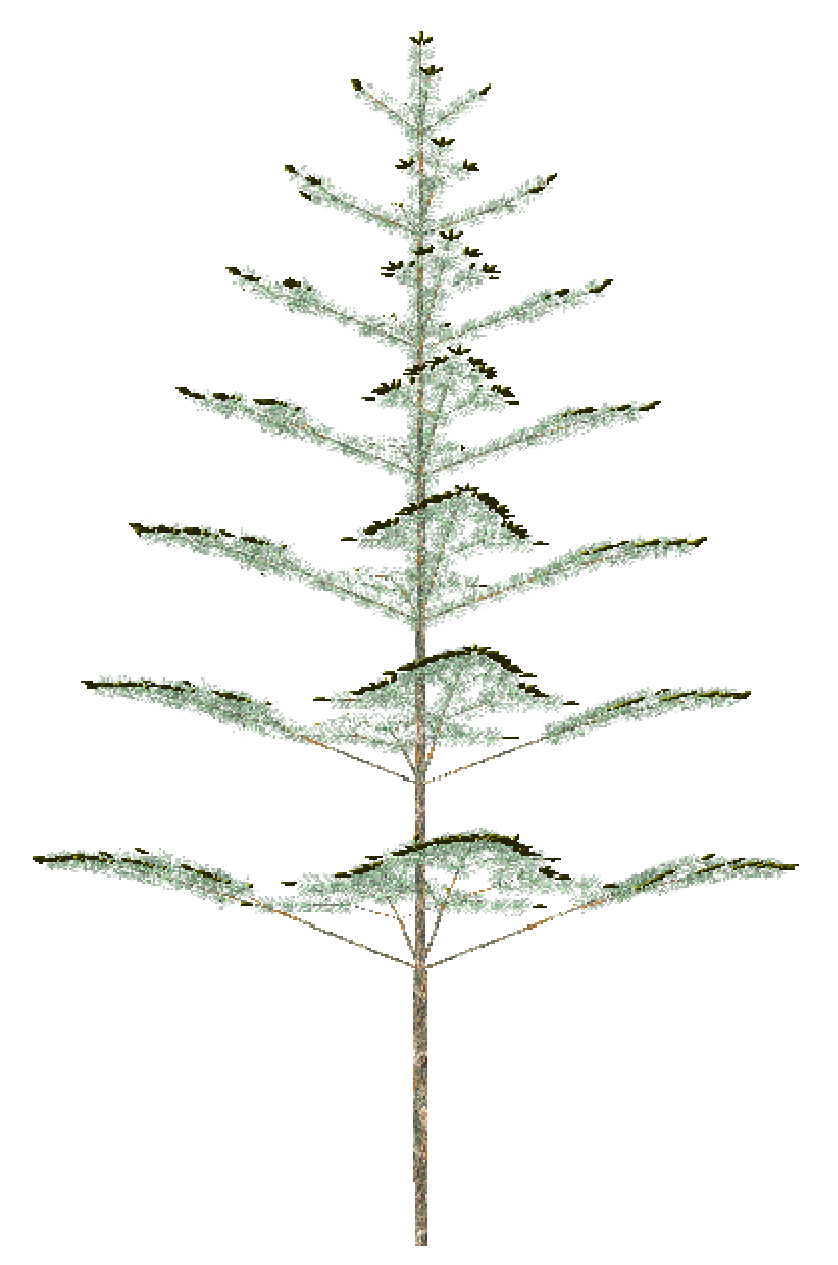
\includegraphics[scale=0.25]{pineL8}
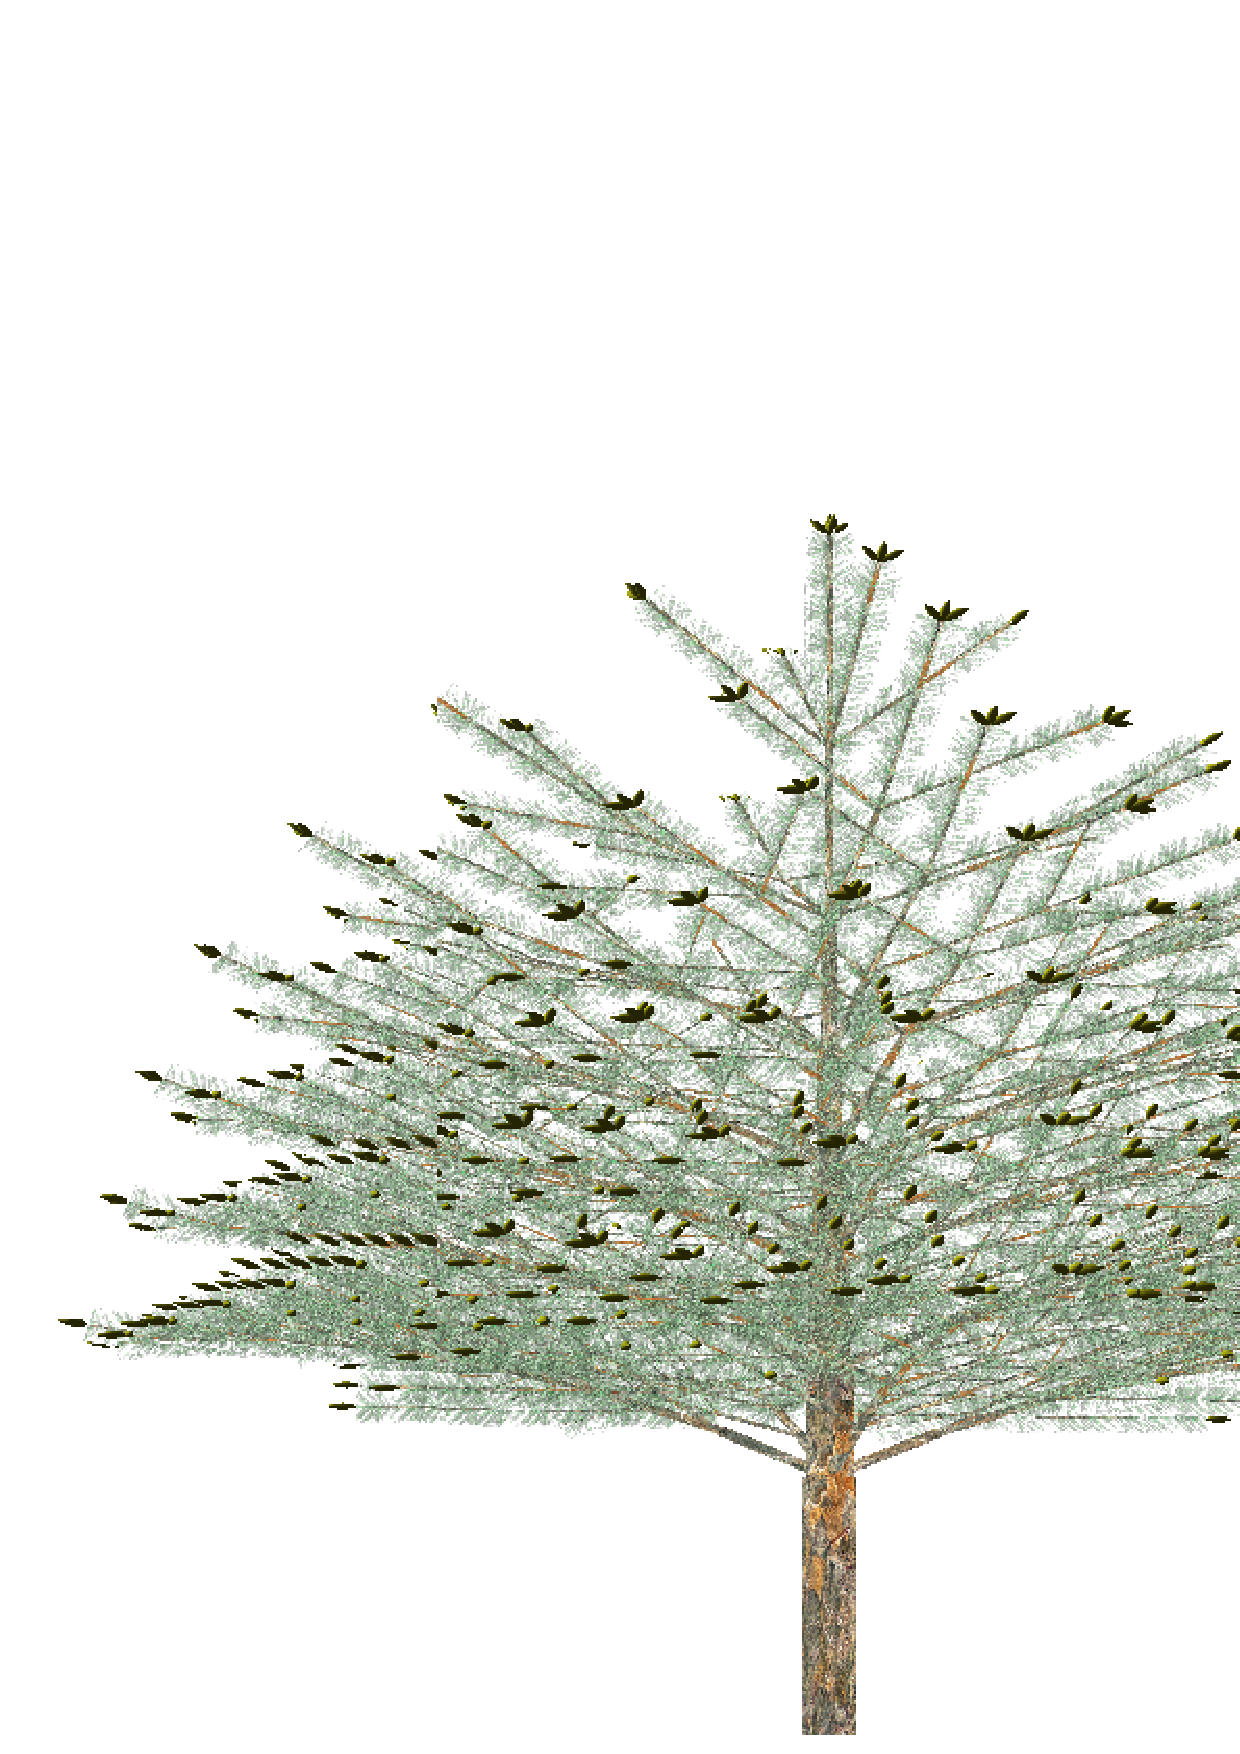
\includegraphics[scale=0.20]{pine8FEM98}
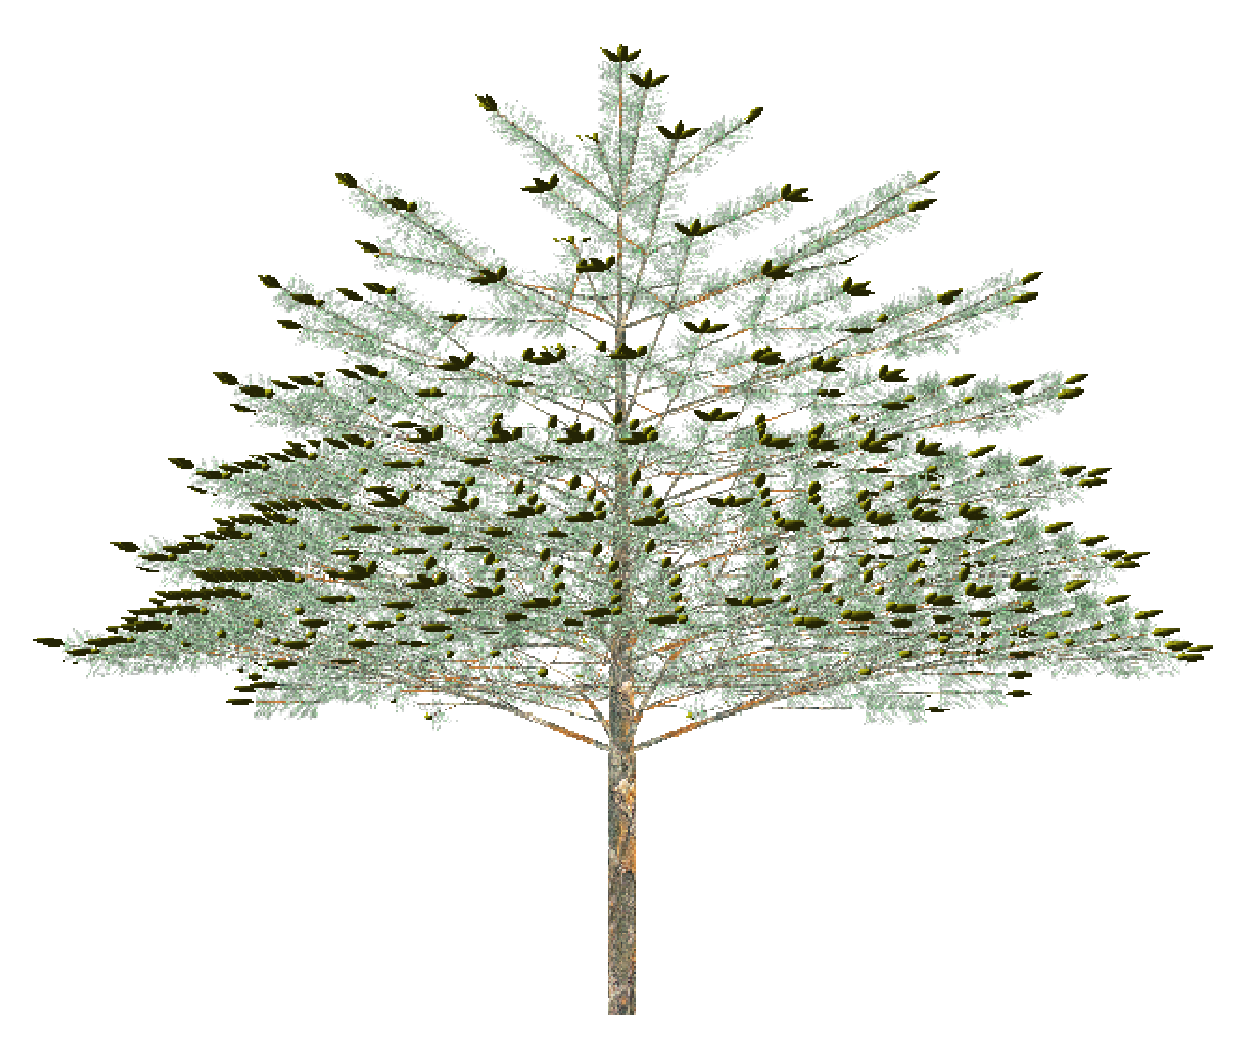
\includegraphics[scale=0.20]{pine8F1}   
\caption{The development of three  pines after eight development steps
when architectural  development is according to L  program of Appendix
\ref{sec:L1} and  metabolic functioning is  as in \citet{perttunen:96,
perttunen:98}. We  omit some functions  of LIGNUM, e.g. the  number of
secondary buds  as a function foliage  mass of mother  segment and let
the L-system determine  branching.  Leftmost: Development according to
L program only, middle and right: interaction of L language and LIGNUM
depicting the effect of  foliage mortality.  Middle: Foliage remains 5
years.  Length  = 3.5  m, diameter  at base =  10 cm.   Right: Foliage
remains 1 year.  Length = 2.7 m, diameter at base 6 cm.}
\label{fig:pine}
\end{figure}


\section{Fragmentary  L system   for  bearberry  growth}\label{sec:L2}

Fragmentary L system for  bearberry growth. The $Start$ module creates
the initial  plant.  The  $B$ module, line  15, checks  for collision.
Lines  18--40   determine  branching  and  growth.    The  pattern  of
ramification is  based on  field data and  implemented in  the uniform
random variables $r1~\mathrm{and}~r2  \in [0,1]$.  $r1$ intializes the
branching to the  left or right.  Branching and  growth depends on the
bud type,  its status and the value  of $r2$.  The counter  on line 41
eventually activates dormant buds ($s > 0$).  Bud types: D = dominant,
N  = nondominant  and  S =  subdominant.   See \citet{salemaa:02}  for
details.

%\begin{figure}[p]
%\begin{picture}(1,1)
%\put(0,0){\line(1,0){370}}
%\end{picture}
\begin{verbatim}
 1.open Bearberry;
 2.const PI = 3.1415926535897932384;
 3.module B(double type,double status,double collision); 
 4.derivation length: 15;
 5.Start:{produce F(0.1) SB() EB() B(D,0.0,0.0);}
 6.B(T,s,C):
 7.{
 8.  double g = 0.0;
 9.  double r1 = ran();
10.  double r2 = ran();
11.  if (r1 < 0.5) 
12.     g = -5*PI/180;
13.  else 
14.     g =  5*PI/180;
15.  if (C == 1.0){
16.    produce B(T,s,C);
17.  }
18.  else if (T == D && s == 0.0){
19.    if (r2 < 0.26)
20.      produce Turn(g)F(0.6)SB()Turn( 30*PI/180)B(N,2,C)EB() 
21.              Turn(g)F(0.1)SB()Turn(-30*PI/180)B(N,1,C)EB()
22.              Turn(g)F(0.1)SB()Turn( 30*PI/180)B(S,1,C)EB()
23.              Turn(g)F(0.1)SB()Turn(-30*PI/180)B(S,0,C)EB()
24.              Turn(g)F(0.1)SB()EB()B(D,0,C);
25.    else if (r2 <= 0.52)
26.      produce Turn(g)F(0.6)SB()Turn(-30*PI/180)B(N,2,C)EB() 
27.              Turn(g)F(0.1)SB()Turn( 30*PI/180)B(N,1,C)EB()
26.              Turn(g)F(0.1)SB()Turn(-30*PI/180)B(S,1,C)EB()
28.              Turn(g)F(0.1)SB()Turn( 30*PI/180)B(S,0,C)EB()
29.              Turn(g)F(0.1)SB()EB()B(D,0,C);
30       ......................................................
32.  } 
33.  else if (T == S && s == 0.0){
33.    if (r2 < 0.037)
34.      produce Turn(g)F(0.48)SB()Turn(-30*PI/180)B(S,1,C)EB()
35.              Turn(g)F(0.08)SB()EB()B(S,0,C);
36.       ......................................................
37.  }
38.  else if (T == N && s == 0.0){
39.       ......................................................
40.  else{
41.    produce B(T,max(s-1,0),C);
42.  }
43.}
44.close Bearberry;
\end{verbatim}
%\begin{picture}(1,1)
%\put(0,0){\line(1,0){370}}
%\end{picture}
%\caption{)
%\end{figure}


\begin{figure}
%\makebox[\textwidth]{\framebox[10cm]{\rule{0pt}{250pt}}} 
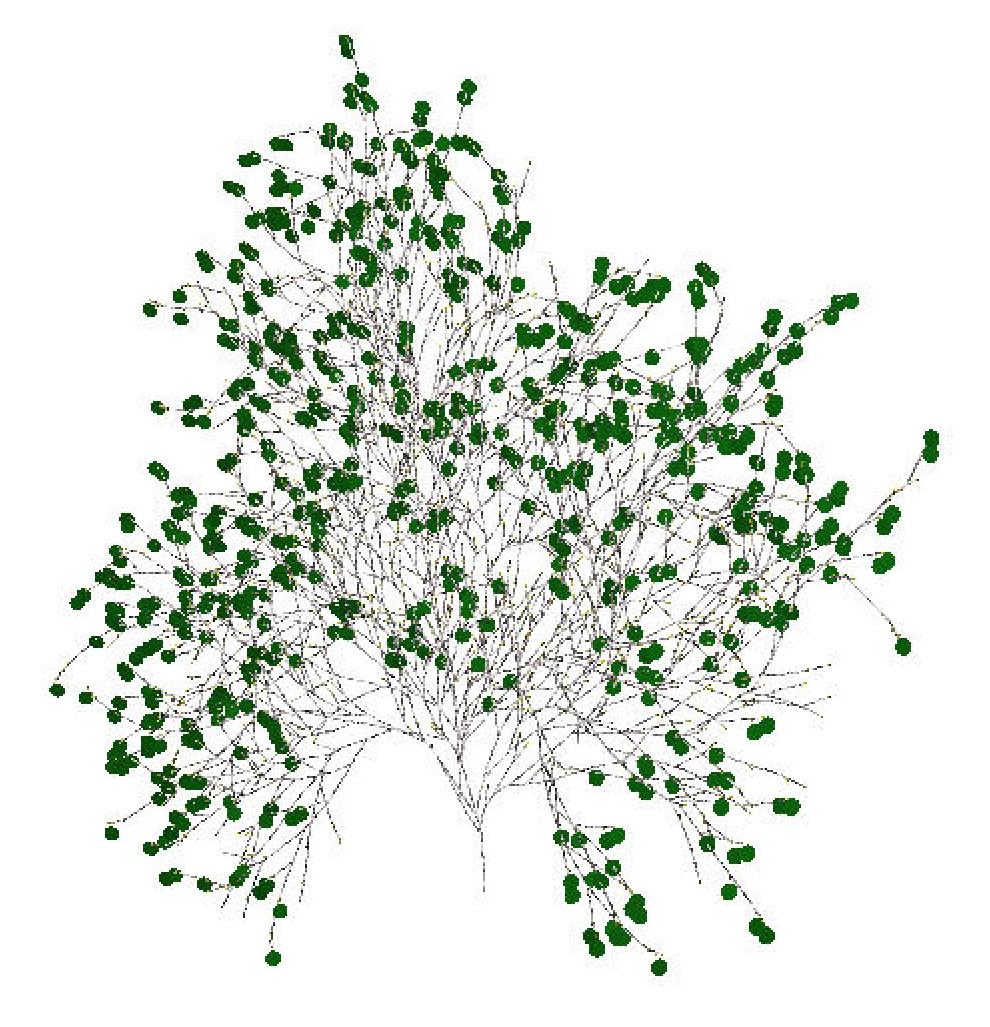
\includegraphics[scale=0.2]{a-uvaursi-15-35-30}
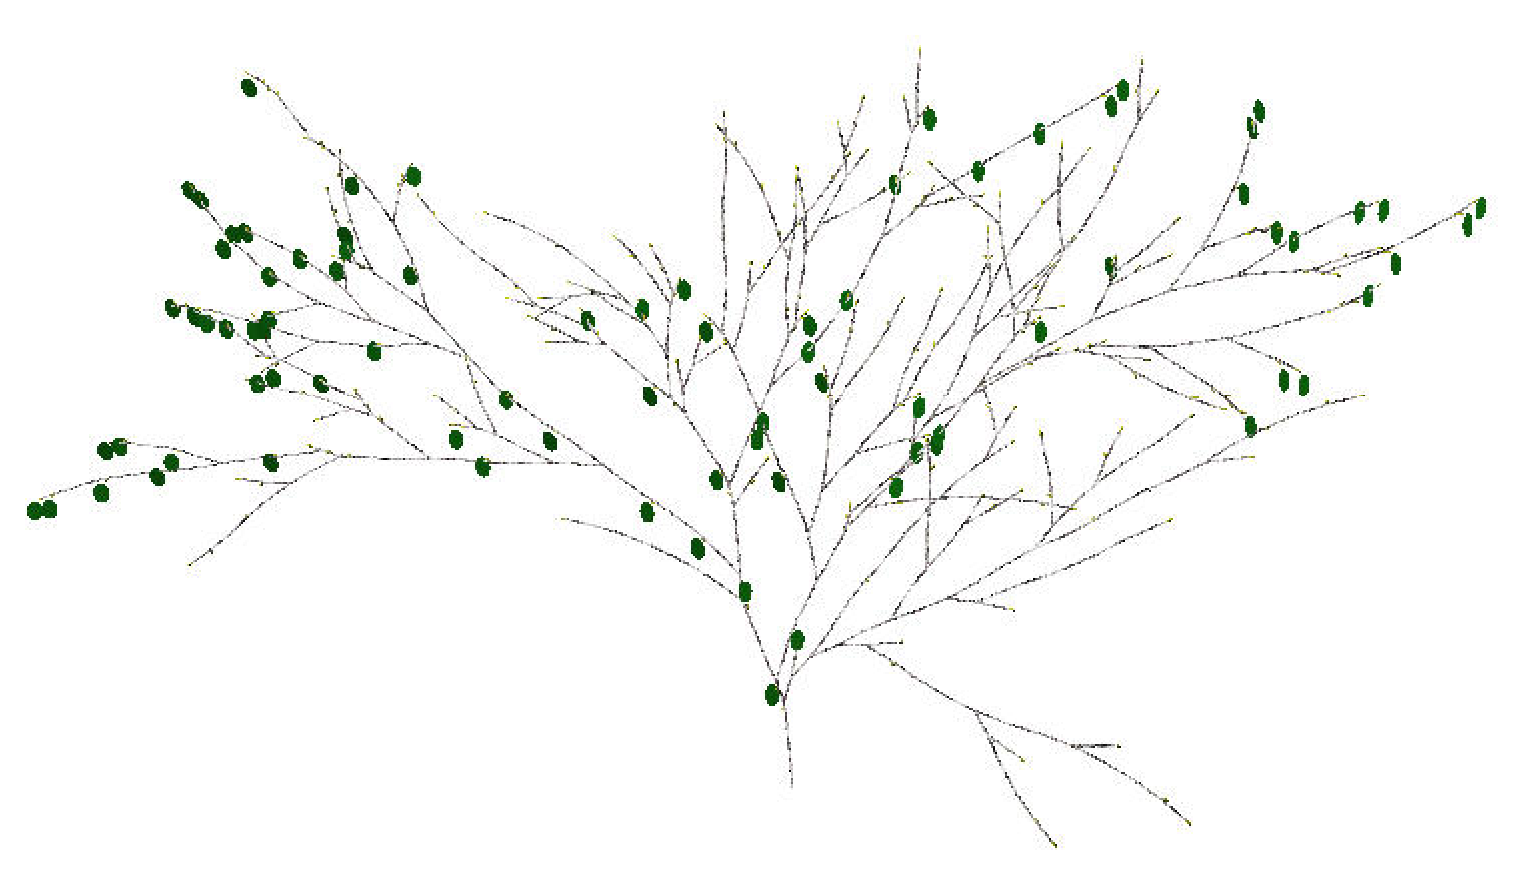
\includegraphics[scale=0.2]{a-uvaursi-15-55-30}
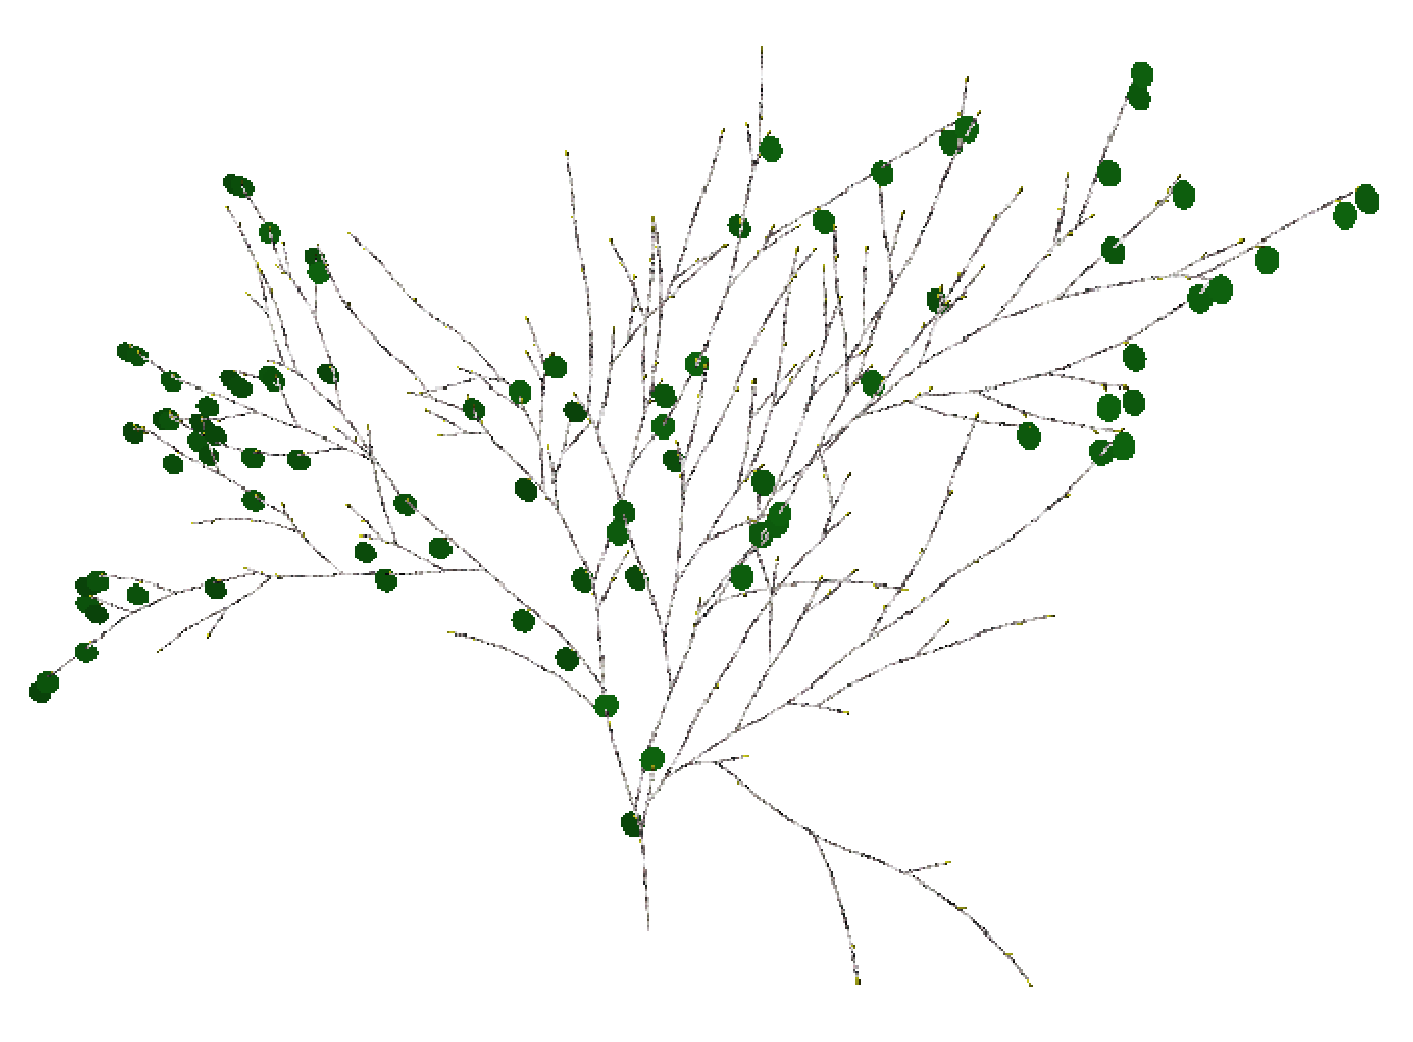
\includegraphics[scale=0.2]{a-uvaursi-15-65-30}    
\caption{Bearberry model after 15 iterations. From left to right 
  opening angle and the distance to obstacle are $35^{\circ}/30\mathrm{cm}, 
 55^{\circ}/30\mathrm{cm}$ and $65^{\circ}/20\mathrm{cm}$.}\label{fig:a-uva-ursi} 
\end{figure}

\begin{figure}[p]
\begin{picture}(1,1)
\put(0,0){\line(1,0){370}}
\end{picture}
\begin{verbatim}   
 V < F(s,A,v):{F(s,A,v)V;}
 F(s,A,v) < V > SB()F(s1,A1,v1)EB() SB()F(s2,A2,v2)EB() F(s3,A3,v3):
 {
    double A_max = max(A1,A2,A3);
    v1 = (A1/A_max)*v;
    v2 = (A2/A_max)*v;
    v3 = (A3/A_max)*v;
    produce;
 }
\end{verbatim}
\begin{picture}(1,1)
\put(0,0){\line(1,0){370}}
\end{picture}
\caption{Vigor index in L-system. For the definition 
         of left and right context in axial trees 
        see \citet{pp:96}.}\label{fig:vi} 
\end{figure}

\end{document}


